%-------------------------------------------------------------------------------
% TEMPLATE FOR UCL MSc ECONOMICS THESES
% (c) Elliott Christensen, 2023

% This is a template for a MSc Thesis document based upon a template uploaded by Sofia Feist, 2020.
%------------------------------------------------------------------------------- 





% ------------------ DOCUMENT SETUP ------------------ 
% The document class defines the document type (article) and sets the font size (12pt)
\documentclass[12pt]{article}

% Your name
\author{Filip Topic}

% Inputs the Document Packages
\input{Packages}

% Controls how many subsections the document can take
%  and how many of those will get put into the contents pages.
%\setcounter{secnumdepth}{2}
% \setcounter{tocdepth}{2}

% Line Spacing
\setstretch{1.5}

% The folder path where the images will be uploaded
\graphicspath{ {./Image/} } 

% Places a dot after Chapter/Section/Subsection number in Table of Contents
% \renewcommand{\cftchapaftersnum}{.}
\renewcommand{\cftsecaftersnum}{.}
\renewcommand{\cftsubsecaftersnum}{}

%  Customize Dot spacing in Table of Contents/List of Figures/Tables
\renewcommand{\cftdotsep}{0.3}

% Numeration Type for Chapters and Sections (Roman I, II, II / Arabic 1, 2, 3)
% \renewcommand\thechapter{\Roman{chapter}}
\renewcommand\thesection{\arabic{section}}

% Line Break Properties
\tolerance=1
\emergencystretch=\maxdimen
\hyphenpenalty=10000
\hbadness=10000


% Formatting Table of Contents/Lists titles
\renewcommand{\contentsname}{\normalfont\bfseries\LARGE{CONTENTS}}
\renewcommand{\listfigurename}{\normalfont\bfseries\LARGE{LIST OF FIGURES}}
\renewcommand{\listtablename}{\normalfont\bfseries\LARGE{LIST OF TABLES}}


% Title Formatting customization
\titleformat{\chapter}{\normalfont\bfseries\LARGE}{\thechapter.}{1em}{\MakeUppercase}
\titlespacing*{\chapter} {0pt} {0pt} {0pt} % left, before, after

\titleformat{\section}{\normalfont\bfseries}{\thesection.}{1em}{\MakeUppercase}
\titlespacing*{\section} {0pt} {0pt} {0pt}

\titleformat{\subsection}{\normalfont\bfseries}{\thesubsection}{1em}{}
\titlespacing*{\subsection} {0pt} {10pt} {10pt}

\titleformat{\subsubsection}{\normalfont\bfseries}{}{1em}{}
\titlespacing*{\subsubsection} {0pt} {10pt} {10pt}


% HEADER AND FOOTER
\pagestyle{fancy}  % Set Page Style (Header and Footer Style)
\fancyhf{}  % Clears the header and footer (from the default info)

% Add a horizontal line by removing the % sign before the renewcommand (or vice versa): 
\renewcommand{\headrulewidth}{0.1pt}

% Header
\fancyhead[L]{\textit{Filip Topic}}
\fancyhead[C]{\textit{MSc Banking and Digital Finance}}
\fancyhead[R]{\textit{September 2024}}

% Footer
\fancyfoot[C]{\thepage} % Page Number

% Change figure numbering per section
\numberwithin{figure}{section}
\numberwithin{table}{section}




%  -------------------------------------------------
%  --------- The document starts from here --------- 
%  -------------------------------------------------

\begin{document}

% ------------------  TITLE PAGE -------------------
\begin{titlepage}
\begin{center}
    % UCL IMAGE
    \vspace*{-3.5cm}
    % Choose colour from the Image Folder: More can be found here: https://imagestore.ucl.ac.uk/imagestore/start/ucl-banners/For%20PRINT/UNCOATED/DL%20PORTRAIT?fc=browse&column=5
    \makebox[\textwidth]{\includegraphics[width=211mm]{Image/ucl-banner-dl-port-darkred-u.eps}}
    \vfill % Elastic empty space filler
    
    % Title
    {\LARGE\textbf{Time-Series Foundation Models (TSFMs) in Finance\\
    % Subtitle
    Do TSFMs outperform traditional Time-Series prediction models in the field of Finance?\\}}

    \vspace{0.8cm}
    by\\
    \vspace{0.8cm}

    % Author
    {\LARGE\textbf{Filip Topic\\}}
    % Date
    \vspace{1.5cm}
    {\Large\textbf{September 2024}}

    \vfill

    \textbf{\setstretch{2.0} 
    Dissertation Supervisor: Ramin Okhrati\\
    \vspace{1cm}
    Dissertation submitted in part fulfilment of the\\
    Degree of Master of Science in Banking and Digital Finance\\
    \vspace{1cm}
    Institute of Finance and Technology\\
    University College London\\}

    \vspace{2cm}
\end{center}
\end{titlepage}
% -------------------  Declaration  ---------------------
\newpage
\include{Declaration}

% ------------------  TABLE OF CONTENTS --------------------
\tableofcontents 



% -------------------  LIST OF FIGURES --------------------
\newpage 
%{\let\oldnumberline\numberline       % Uncomment to add the word 'Figure' to figure number in List of Figures
%\renewcommand{\numberline}{\figurename~\oldnumberline}  
\listoffigures%}
\addcontentsline{toc}{section}{List of Figures} % Add List of figures into contents without any numeration 



% -------------------  LIST OF TABLES ---------------------
\newpage
\listoftables 
\addcontentsline{toc}{section}{List of Tables} % Add List of tables into contents without any numeration 



% -----------------  ACKNOWLEDGEMENTS  -------------------
\newpage
\section*{Acknowledgements}
\addcontentsline{toc}{section}{Acknowledgement}


% ----------------------  ABSTRACT -----------------------
\newpage
\section*{Abstract} % the Asterix (*) indicates that this section will be added to the table of contents but no number will be present beside it.
\addcontentsline{toc}{section}{Abstract}

\newline
\newline
\textbf{Keywords:} 


% -------------------  INTRODUCTION  ---------------------
\newpage
\section{Introduction} 

\subsection{Time-Series prediction}
Since the beginning of financial markets, their participants have had the desire to predict the future values of instruments being traded there. And for this purposes, they have used many different techniques - majority of which have fallen short of randomly guessing the direction of the price movement. In the past few decades, many models have emerged which claim excellent capability of time-series prediction. First were the statistical models (such as ARIMA), then the Machine Learning models (such as XGBoost), then Deep Learning models (such as DeepAR). 

\subsection{Transformer-based Models}

The revolution in the field of Machine Learning came in 2017 with the invention of the Transformer architecture (more specifically: the attention mechanism). Transformer based models have taken the whole field of ML by storm, however, their application has mostly been in the sub-field of Natural Language Processing. Recently they started seeing use in the field of time-series prediction (eg. Informer). 

\subsubsection{Time Series Foundation Models (TSFM)}

Time-series foundation models are large transformer-based models which are designed for the purpose of time-series prediction and which have been pre-trained on a large amount of time-series data. This research will explore their use on financial time-series data





% ---------------  BACKGROUND -----------------
\newpage
\section{Background} 

\subsection{The Transformer}

In 2017, Vaswani et al. \cite{vaswani2017attention} introduced a ground-breaking model called the "Transformer". Transformer is a model designed to solve the sequence-to-sequence mapping problem. In a sequence-to-sequence problem we have a sequence which consists of tokens\footnote{A token is a multi-dimensional numeric vector representation of an element in the sequence. Reason why sequence of tokens is used as input to a sequence-to-sequence model is because ML models can only "understand" numbers - therefore they can't work with some type of sequences (eg. human language sentences). Reason why tokens are vectors rather than simple nubers is because they are designed to represent the semantic meaning of a real-world element they represent and the semantic meaning of a real-world element could change depending on the context. Therefore different dimensions of a token account for different meaning of that element in different contexts.} coming from a finite vocabulary\footnote{The vocabulary doesn't always need to be finite, as we will see later on.} which are in a specific order, and we have an output sequence which is again a sequence of tokens in a specific order. The task of a sequence-to-sequence model is to learn the correct relationship between the input and output sequences so that when the model is presented with an unseen input sequence, it can predict what the correct output sequence is. In essence, sequence-to-sequence model's goal is to learn the "meaning" of the relationship between the input and output sequence. An example of sequence-to-sequence tasks are:
\begin{enumerate}
    \item Language translation - where an input sequence could be a sentence in our native language and the output sequence would be the correct translation of that sentence in a foreign language.
    \item Chatbots - where an input sequence could be a question and the output sequence the correct answer to that question.
    \item Time-series forecasting - where an input sequence is a certain time-series and the output sequence is the future values of that time-series. 
\end{enumerate}

Before the Transformer, there have been many ML models which attempted to solve these tasks. Sutskever et al. (2014) \cite{sutskever2014sequence} used multilayer LSTM\footnote{LSTM stands for Long Short Term Memory cell} (type of RNN\footnote{RNN stands for Recurrent Neural Network. It is a type of Artificial Neural Network architecture.} model) for this task. LSTM \cite{hochreiter1997long} and GRU\footnote{GRU stands for Gated Recurrent Unit. GRU is also a type of RNN.} \cite{cho2014learning} used to be state-of-the art sequence-to-sequence models, however they have some key issues. They require large memory\footnote{This means that it is difficult to parallelize the training process across training examples and smaller batch sizes had to be used.}, their nature is sequential\footnote{This means that it is impossible to parallelize training within the training examples.}, and they suffer from an information bottleneck due to the fixed size of the hidden state\footnote{The hidden state is an intermittent sequence within a sequence-to-sequence model. It is a product of applying the encoder on the input sequence. The output sequence is generated by applying the decoder to the hidden state. Having a hidden state of fixed size means that some information will inherently get lost when a very long input sequence is fed into the model.}. These problems were adressed by the Transformer.

\begin{figure}[h]
\centering
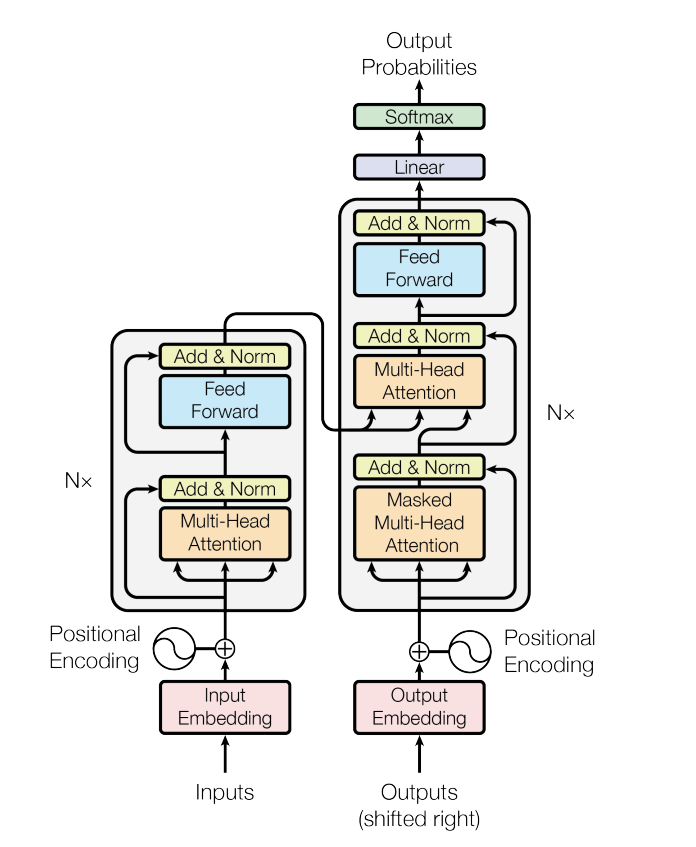
\includegraphics[width=8cm]{transformer.PNG}
\caption{Transformer architecture schema \cite{vaswani2017attention}}
\label{fig:transformer}
\end{figure}

Transformer consists of and Encoder and a Decoder\footnote{Similar to already mentioned RNNs.}. Figure \ref{fig:transformer} is a schematic representation of the Transformer model. Left part is the Encoder and the right part is the Decoder.

\subsubsection{Encoder}

The encoder is a stack of multiple identical layers\footnote{In the original paper there are 6 of these layers in the encoder stack}, each layer consisting of two sub-layers:

\begin{enumerate}
    \item Multi-head self-attention layer
    \item Feed-forward neural network
\end{enumerate}

Multi-head Self-attention layer consists of N so-called "attention heads"\footnote{In the Original paper, N = 8.}. An attention head is essentially a series of arithmetic operations performed on the input sequence: Let's say we have a sequence of tokens S = {s\textsubscript{1}, s\textsubscript{2}, ..., s\textsubscript{n}} the dimension of input tokens is 1 x d\textsubscript{model} \footnote{In the original paper, d(model) = 512.}. An attention head consists of weight matrices\footnote{These weight matrices are all learnable weights.} W\textsuperscript{Q}, W\textsuperscript{K} and W\textsuperscript{V} \footnote{Q, K, and V stand for Query, Key and Value.} of the dimension (d\textsubscript{model} x d\textsubscript{k}) where d\textsubscript{k}=d\textsubscript{model}/N. Multiplying these weight matrices by token s\textsubscript{i} from the input sequence creates Q\textsubscript{i}, K\textsubscript{i} and V\textsubscript{i} vectors respectively of dimension 1 x d\textsubscript{k}. For each token i, dot product of Q\textsubscript{i} and K\textsubscript{j} (for all j, 0<j<n+1) is calculated: dot\textsubscript{i, 1}, dot\textsubscript{i, 2}, ..., dot\textsubscript{i, n}. These dot-products are then scaled\footnote{Scaling factor is 1 / square root of d(k). According to the paper, this is done so that the weights are more stable during training.}, a softmax layer is applied\footnote{Applying Softmax on a series of numbers means scaling all of them so that they sum up to 1.} to all these dot products. Each dot product dot\textsubscript{i, j} then multiplies the corressponding V\textsubscript{j} to get the series of V vectors: V\textsubscript{i, 1}, V\textsubscript{i, 2}, ..., V\textsubscript{i, n}. All these V vectors are then element-wise summed up to Z\textsubscript{i} (of dimension 1 x d\textsubscript{k}) which represents the self-attention output for the token i. This is repeated for all n tokens and creates a series of vectors Z\textsubscript{1}, Z\textsubscript{2}, ..., Z\textsubscript{n} (one for each token) which are then vertically stacked into matrix Z of dimension n x d\textsubscript{k}. This matrix Z\textsubscript{h} is the output of the single self-attention head h. If we vectorize this process\footnote{When we need to do the same arithmetic operations multiple times with different vectors, we can simply concatenate these vectors into matrices and do the operations just once with these matrices.}, we can express attention as \[\text{Attention}(Q, K, V) = \text{softmax}\left(\frac{QK^T}{\sqrt{d_k}}\right) V\]
 See Figure \ref{fig:scaleddotproductattention}:

\begin{figure}[h]
\centering
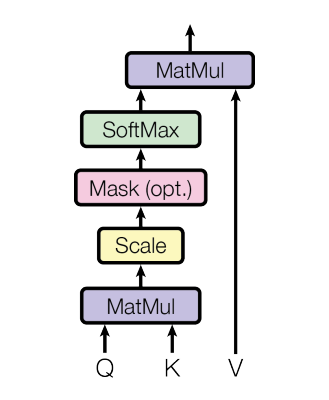
\includegraphics[width=6cm]{Image/scaled dot product attention.PNG}
\caption{Scaled Dot product attention \cite{vaswani2017attention}}
\label{fig:scaleddotproductattention}
\end{figure}


This process goes on in parallel in every head of the multi-head self-attention layer. Finally, the Z matrices of each self-attention head Z\textsubscript{1}, Z\textsubscript{2}, ..., Z\textsubscript{N} are horizontally concatenated to produce the output of the whole multi-head self-attention layer L: Z\textsubscript{L} (of dimension n x N*d\textsubscript{k}. Multi-head self-attention layer has a weight matrix W\textsubscript{O} of dimension N*d\textsubscript{k} x d\textsubscript{model} which gets multiplied by Z\textsubscript{L} to produce the final output of the multi-head self-attention layer L.

Before the output of the multi-head self-attention layer goes into a feed-forward neural network\footnote{This network has two hidden layers with ReLU actiavation of the first layer and linear activation of the 2nd layer. In the original paper, dimensionality of hidden layers is 2048.}, a residual connection\footnote{Residual connection in this context means adding the input of the layer to the output of that layer before passing to the next layer. This is used to mitigate the vanishing gradient problem and to stabilize the training process.} \cite{he2016deep} and layer normalization\footnote{Layer normalization is a scaling technique that normalizes the the data across features within each data-sample indivisdually, as opposed to batch normalization which normalizes each feature across multiple data-samples.} \cite{ba2016layer} are applied. Residual connection and layer normalization are applied after every sub-layer of the Encoder and Decoder.  

\subsubsection{Decoder}

The Decoder has a similar structure as the Encoder with a few notable differences.

Same as the Encoder, Decoder has N layers. Each layer has three sub-layers: 

\begin{enumerate}
    \item masked self-attention layer
    \item encoder-decoder attention layer
    \item feed forward layer
\end{enumerate}
 
In principle, masked self-attention layer works similarly as the multi-head attention layer in the Encoder, however, Q, K, and V come from the already generated output\footnote{This makes the Decoder particularly suitable for autoregressive tasks as it predicts tokens sequentially based on which tokens have been predicted before, as opposed to the Encoder which would predict a sequence of tokens which it thinks would have the highest probability of being true overall without regard for the order of the sequence.}, and the attention is calculated only for the current and previously generated outputs i.e. for an already generated token i, masked self-attention head only calculates Z\textsubscript{1}, Z\textsubscript{2}, ..., Z\textsubscript{i}. Otherwise, the process is the same as in the Encoder multi-head self-attention sub-layer\footnote{i.e. Encoder also stacks the outputs of each head, applies the Wo matrix, the residual connection and layer normalization.}. (See Figure \ref{fig:transformer}.)

Encoder-decoder attention layer also works similarly as the multi-head self-attention layer in the Encoder, however in this layer Q comes from the previous masked self-attention layer but K and V come from the Encoder. This allows every position in the Encoder to attend all positions in the input. (See Figure \ref{fig:transformer}.)


\subsubsection{Summary}

Even though the Attention mechanism has been around for a while \cite{bahdanau2014neural}, the self-attention model, as implemented in the Transformer, was a revolutionary step - as it solved the issue of long range dependancies\footnote{Earlier attention models had issues relating tokens which were too far apart due to attention being applied only on hidden states (hidden states are a feature of RNN models) rather than on inputs directly.}. This concept enables the model to learn the intrinsic structure of the sequence it is presented with and therefore builds a certain level of actual "understanding" of the inputs rather than simple "fitting". 

Another revolutionary aspect of the Transformer is the positional encoding. Positional encoding injects information about the absolute and relative position of each token in the sequence\footnote{this is done by sumating each input token with a positional vector of equal dimension. Value of each number in the positional vector is a sin (or could be cos) function of the position of the token it is being added to as well as of the position inside the positional vector.} thus allowing the model to learn about the importance of relative positions of tokens\footnote{This is most important on the field of NLP (Natural Language Processing) tasks.}.

Finally, and probably most importantly, the way Transformer processes inputs is inherently parallelizable - allowing significant scaling benefits to be exploited and very large models to be built. This is beneficial as larger models can learn more intricate patterns in the data and they allow for richer vector representations of the input data\footnote{Vector representations in the original Transformer had the dimension 512, whereas some modern transformer-based models support dimensions in the thousands.} \footnote{Richer representations of the input data means that the model is able to better understand more nuanced differences between some similar input tokens.}

\subsection{Transformer-based models}

Many have built on the success of the Transformer and have come up with their own models which retain many concepts from the original Transformer.

\subsubsection{NLP Transformer-based models}

Among the most famous NLP transformer-based models are the BERT (2018) \cite{devlin2018bert}, T5 (2019) \cite{roberts2019exploring} which themselves have been built upon many times (2019 alBERT \cite{lan2019albert}, 2019 roBERTa \cite{liu2019roberta}, 2019 distilBERT \cite{sanh2019distilbert}, 2020 mT5 \cite{xue2020mt5}, 2024 flan-T5 \cite{chung2024scaling}), however, OpenAI's GPT\footnote{GPT stands for Generative Pre-trained Transformer} series and LLaMA series \cite{touvron2023llama} take the crown as the most famous Transformer-based NLP models by far.

\subsubsection{CV (computer vision) Transformer-based models}

Among the most famous CV transformer-based models are 2020 ViT \cite{dosovitskiy2020image}, 2020 DETR \cite{carion2020end}, and 2021 swin-Transformer \cite{liu2021swin}.

\subsubsection{Speech and Audio processing Transformer-based models}

\subsubsection{Time-series Transformer-based models}

It was a matter of time Transformer-based architectures appeared in time-series prediction tasks. Li et al. (2019) \cite{li2019enhancing} wrote a pioneering work on transformers (LogSparse Transformer) in time-series forecasting where they adressed the issue of the quadratic space complexity\footnote{Quadratic space complexity of a model means that the ammount of working memory a model uses grows quadratically with the size of the input of the model. This is especially problematic for longer inputs for which the required memory could explode.} of the Transformer\footnote{They used heuristic approach to reduce the storage complexity to O(L*log(L)).} and proposed a more task-appropriate version of self-attention\footnote{They proposed so-called "convolutional self-attention" which brings local context awareness to Q-K mathcing}. Zhou et al. (2021) \cite{zhou2021informer} proposed a model (Informer) which also reduces computational and space complexity to O(L*log(L)) using "ProbSparse" self-attention mechanism\footnote{ProbSparse self-attention uses Query Sparsity Measurement - a metric which helps determine which Qs are more "dominant" so that the attention can be calculated for only those Qs. This is an upgrade from LogSparse Transformer, which used a heuristic to determine Which QK pairs will be calculated.} and self-attention distilling\footnote{Distilling means that the outputs of each the self-attention layers are smaller than their inputs - thus reducing the number of calculations in every subsequent layer relative to the previous one.}. Zhou et al. (2021) \cite{zhou2022fedformer} incorporate a seasonal-trend decomposition approach \cite{cleveland1990stl} \cite{wen2019robuststl}, along with Fourier analysis into the transformer-based model (FEDformer)\footnote{FED stands for Frequency Enhanced Decomposition.}. This approach saw great improvements in time-series prediction. Improvements were in terms of lower prediction errors as well as in terms of the distribution of predictions being closer to the distribution of ground-truth values according to the Kolmogorov-Smirnov distribution test\footnote{Authors of the FEDformer claim even though Informer predictions were good, they don't have the same distribution as the ground-truth time-series.} \cite{massey1951kolmogorov}.


\subsection{Time-series Foundation models (TSFM)}

Foundation Models (FM) are a class of deep models which are pre-trained on a large ammount of data - thus being able to generalize\footnote{Generalization is the ability of a model to perform well on data that it hasn't been trained on.} well as they have been taught many diverse patterns. FMs saw success on the fields of CV and NLP so it is only natural that development of FMs start developing on the time-series front. And so was the case: Since 2022, over 50 models, which can be classified as Time-series Foundation Models, have been released. If we analyze the TSFM landscape, according to the taxonomy proposed by Liang et al. (2024) \cite{liang2024foundation}, we can see that the TSFM is a very diverse class of models. TSFMs can be classified according to:

\begin{itemize}
    \item Type of time-series it is working with, which can be:
    \begin{enumerate}
        \item Standard time-series\footnote{Standard time-series is a simple sequence of any number of data-points, each associated with a time-stamp, ordered chronologically.}.
        \item Spatial time-series\footnote{Spatial time-series is a standard time-series but with a spatial dimension as well.}.
        \item Trajectory\footnote{Trajectory is a sequence of time-stamped locations which describe the movement of an object in space.}.
        \item Event sequence\footnote{Event sequence is a chronologically ordered sequence of events within a specific context.}.
    \end{enumerate}
    \item Model architecture, which could be:
    \begin{enumerate}
        \item Transformer-based.
        \item Non-Transformer-based\footnote{These models are usually MLP, RNN or CNN -bases models.}.
        \item Diffusion-based \cite{sohl2015deep} \cite{ho2020denoising}\footnote{Diffusion-based models are self-supervised models usually applied in image generation. They are trained by adding gaussian blur to the training-sample in a markov process manner and then applying (usually) CNN-based model to learn how to un-blur the same sample.}.
    \end{enumerate}
    \item The nature of the models' pre-training. which could be:
    \begin{enumerate}
        \item Pre-trained LM (Large Model)\footnote{These models use a model (usually Large Language Model) which has already been trained on some other type of sequential data, for another task and they just adopt it for time-series. Adoption strategies usually involve changing the way the inputs are tokenized in order to work better with time-series data.}.
        \item Self-supervised\footnote{Self-supervised models can be further split into Generative, Contrastive and Hybrid models. Generative models are those which have been trained to reconstruct the input data. They are particularly useful for tasks that involve generating a "missing" part of the input data (such as time-series forecasting). Contrastive models are those that have been trained to distinguish between "similar" and "dissimilar" pairs of data. As such, they are more appropriate for classification tasks (In time-series analysis, they are usually used for anomaly detection). As the name suggests, Hybrid models use mix of these two strategies.}.
        \item Fully supervised.
    \end{enumerate}
    \item Capabilities to adapt to a new time-series, which could be:
    \begin{enumerate}
        \item Fine-tuning.
        \item Zero-shot learning.
        \item Prompt engineering.
        \item Tokenization.
    \end{enumerate}
\end{itemize}

In this dissertation, I will only consider a small subset of TSFMs; ones that belong to a class of standard time-series, Transformer-based, Self-supervised (Generative) models with fine-tuning capability. However, this class of TSFMs is itself very large \cite{liang2024foundation} ( in no particular order: PatchTST \cite{nie2022time}, MOIRAI \cite{woo2024unified}, Lag-Llama \cite{rasul2023lag}, TimeSiam \cite{dong2024timesiam}, Timer \cite{liu2024timer}, TimesFM \cite{das2023decoder}, UniTS \cite{gao2024units}, TimeGPT-1 \cite{garza2023timegpt}, Chronos \cite{ansari2024chronos}, MTSMAE \cite{tang2022mtsmae}) so the efforts of this dissertation will be focused on two pioneering examples, trained on vast collection of time-series data spanning multiple domains \cite{liang2024foundation}: Lag-Llama and TimeGPT-1.





% ---------------  Literature review -----------------
\newpage
\section{Literature review} 


\subsection{TimeGPT-1 \cite{garza2023timegpt}}

TimeGPT-1 is closed-source model - meaning that there is a lot of opacity to model's architecture, parameters and trainng data.

\subsubsection{Architecture}

TimeGPT-1 has encoder-decoder structure with multiple layers, each having residual connections and layer normalization. It utilizes self-attention mechanism based on the original Transformer \cite{vaswani2017attention}. 

Special capability of TimeGPT-1 is multivariate time-series forecasting - meaning that it is able to take into account "special events" and exogenous features\footnote{Special events and exogenous features are time-series which are assumed to have some influence on the target time-series. Example of the former being bank holidays if the target time-series if number of flights per day and example of the latter being price of petrol if we are forecasting number of cars on the road.} when making predictions on a target time-series. However, in order to take full advantage of this feature, we would have to know for certain the realizations of the exogenous variables in the future which is almost never the case in time-series forecasting\footnote{because we can never predict anything in the future with certainty.}. TimeGPT-1 solves this by separately forecasting the exogenous variables into the future and then basing the forecast of the target time-series on its own forecast of the exogenous features. %In my opinion this is a flawed approach, inferior to simple uni-variate prediction as it brings in additional dimensions of uncertainty - whether the exogenous variables forecast are correct and whether the forecasted relationship between exogenous variables and target time-series is correct. One could make a case that 

\subsubsection{Training Data}

Authors claim TimeGPT-1 has been trained on a data-set containing over 100B data-points - the largest collection of publically availible time-series according to their knowledge. Data comes from the domains of finance, economics, demographics, healthcare, weather, IoT sensor data, energy, web traffic, sales, transport, and banking. Due to diversity of data domains, the training set contains time-series with many different characteristics: seasonalities, cycles, trends, noise, outliers. Having been trained on such a diverse dataset, TimeGPT-1 has very strong robustness and generalization capabilities.

\subsubsection{Results}



\subsection{Lag-Llama \cite{rasul2023lag}}

\subsubsection{Tokenization}

Lag-Llama constructs "lagged features" from the past values of the time-series according to a set of frequency-dependant set of lag indices L\textsubscript{indices}={1, ..., N}. The set of lagged features of a point x\textsubscript{t} at timestamp t is then \{x\textsubscript{t-L\textsubscript{indices}[i]}, for all integers i such that 0<i<N+1\}. Lag-Llama also constructs "date-time features" F which for a point x\textsubscript{t} in time t contain information about second-of-the-minute, minute-of-the-hour, ..., month-of-the-year. Final tokenization is done by simply concatenating the date-time features and lagged features into a single vector.

\subsubsection{Architecture}

Lag-Llama is an open-source, decoder-only TSFM based on LLaMA \cite{touvron2023llama} architecture with reduced number of parameters\footnote{ Original LLaMA series comes in sizes of 6.7B, 13.0B, 32.5B and 65.2B parameters.} (2.5m) . Similarly as LLaMA, Lag-Llama utilizes concepts such as RMSnorm \cite{zhang2019root}\footnote{RMSnorm is a layer normalization technique. Zhang and Sennrich (2019) demonstrate that centering component of the LayerNorm technique is dispensable (and computationally expensive) and propose their own layer normalization strategy called RMSnorm which delivers similar benefits (more stable training and better model convergence) but with lower computational cost.}, RoPE \cite{su2024roformer}\footnote{RoPE stands for Rotary Positional Encoding. This is a method for positional encoding. RoPE enables valuable properties, including the flexibility of sequence length,
decaying inter-token dependency with increasing relative distances, and the capability of equipping linear self-attention with relative position encoding.} and SwiGLU \cite{shazeer2020glu}\footnote{SwiGLU activation function is a combination of swish and GLU activation functions. With beta hyperparameter equal to 1, it is of similar shape as ReLU but completely smooth (continuous) - therefore "behaving better" during model training.} activation function\cite{miller2024survey}. On top of N decoder layers, Lag-Llama has a "parametric distribution head". Parametric distribution head is a module which predicts the distribution parameters of the next prediction, given the set distribution. Authors of the paper have chosen student-t distribution for the distribution head, meaning that at inference time, the model predicts the degrees of freedom, mean and scale \cite{student1908probable} of the t-distribution from which it randomly draws n samples - idea being that this sample of n predictions gives a probabilistic insight into the model's prediction. See Figure \ref{fig:lagllama}:

\begin{figure}[h]
\centering
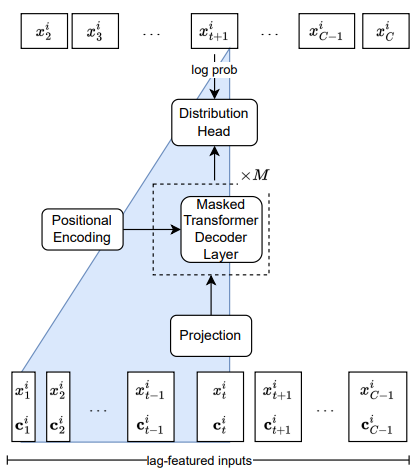
\includegraphics[width=8cm]{Image/lag_llama.PNG}
\caption{Lag-Llama architecture \cite{rasul2023lag}}
\label{fig:lagllama}
\end{figure}

\subsubsection{Training data}

Lag-Llama is pre-trained on diverse set of time-series domains such as energy, transportation, economics, nature, air quality and cloud operations.

% ---------------  METHODOLOGY -----------------
\newpage
\section{Methodology} 

This Research aims to answer 3 main questions:

\begin{enumerate}
  \item How good are TSFMs on financial time-series data?
  \item In which cases do they perform better/worse?
  \item How to improve TSFMs performance?
\end{enumerate}

Methodology of this research is designed in a way to try best answer these three questions in a scientific, statistically significant manner.

\subsection{Time-series prediction evaluation}

Time-series predictions are evaluated using the traditional regression metrics due to the continuous nature of the target variables. All regression metrics are based on some variation of the prediction error\footnote{Prediction error is the difference between the value we predicted and the actual value}. From the prediction error, following metrics are derived, and commonly used in time-series prediction tasks in Finance\cite{hu2021survey}:

\begin{itemize}
  \item RMSE (Root Mean Square Error)
  \item MAE (Mean Absolute Error)
  \item MAPE (Mean Absolute Percentage Error)
  \item R2
\end{itemize}

An additional metric that will be used in this research is MDA (Mean Directional Accuracy)\footnote{MDA is time-series specific. Since time-series data is inherently ordered (as opposed to regular regression data), we can measure the direction in which a time-series is moving at each time-step. Hence we can compare the direction of movement of our predicted time-series against the actual time-series and we can calculate in what percentage of cases did the two time-series move in the same direction (up or down).}. See \cite{costantini2016forecasting} for Directional accuracy calculation.

This is especially important in the field of Finance as in many cases (such as with stock prices) we are not necessarily primarily interested in predicting the actual values, but rather we are interested in predicting the direction in which the price will go next time-step.

\subsection{Data}

This project uses 4 types of financial time-series data:
\begin{enumerate}
  \item Stock index prices
  \begin{enumerate}
      \item S\&P 500
      \item FTSE 100
      \item DOW Jones
      \item NASDAQ
  \end{enumerate}
  \item Exchange rates
  \begin{enumerate}
      \item USD/GBP
  \end{enumerate}
  \item Commodity prices
  \begin{enumerate}
      \item WTI (Oil)
  \end{enumerate}
\end{enumerate}

The specific time-series were chosen solely based on their prominence in the field of Finance.

\subsubsection{Data Pre-processing}

In the field of Finance, there is a concept of "return". Return of an asset A at a certain point in time T: A\textsubscript{T} is calculated as \[(A_T-A_{T-1})/A_{T-1}\] i.e. the percentage change in the value of that asset between the points in time T and T-1. If we think about each one of the fore-mentioned time-series as assets, we can represent them as time-series of returns rather than their actual values which is a common practice in financial time-series prediction \cite{hu2021survey}.


\subsubsection{Time-series data characteristics}




Time-series data exhibits several key characteristics that are essential for effective analysis and forecasting.

\begin{itemize}
    \item Trend\footnote{Trend is a long-term increase or decrease in the data. It could take many shapes: linear, exponential, polynomial, damped.}
    \item Seasonality\footnote{Seasonality is the presence of recurring patterns at regular intervals in the data.}
    \item Noise\footnote{Noise or randomness is short-term fluctuations in the data that do not follow any discernible pattern.}
    \item Stationarity\footnote{A time-series is said to be stationary if the statistical properties such as mean and variance remain constant over time.}
    \item Volatility\footnote{Volatility is degree of variation within the time series.}
    \item Autocorrelation\footnote{Autocorrelation is the degree to which previous values affect future values in a time-series.}
\end{itemize}



Depending on the type and frequency of a financial time-series, it may exhibit different characteristics, therefore, it is important to run experiments across different types of data and different frequencies to find out how well the models handle different time-series characteristics.



\subsection{Experiment Design}

\subsubsection{Benchmark}

Calculating the evaluation metrics for time-series prediction is not sufficient to answer whether a time-series prediction model is good or not. The results of the evaluation need to be put into context and compared against a benchmark in order for us to be able to say whether the results are good or not. 

Chosen benchmark models are: autoARIMA \cite{hyndman2008automatic}\footnote{Originally, this package is for R. I used the equivalent python implementation: https://github.com/alkaline-ml/pmdarima.}, simple autoregressor and Meta's Prophet model \cite{taylor2018forecasting}.

\subsubsection{Time Series Cross Validation}

K-fold Time Series Cross Validation (TSCV) is a statistical method for ensuring statistical significance of a time-series prediction task. In this experiment, I'm using the rolling window version of the TSCV method. Let's say we have chosen the length of the training set to be L, the prediction horizon (how many steps into the future we're predicting) to be H and the time-series of interest has the length L. On the first fold of the TSCV process, we will choose the points 1, 2, ..., L from the time-series to be the "train" set (window) and the points L+1, L+2, ..., L+H to be the "test" set (window) against which we evaluate our models' predictions. (In the field of finance, we are usually only interested in predicting just the next value in the future therefore, in this research, I will use just H=1.) On the next fold of the TSCV, we move the train and test window by one point so we choose points 2, 3, ..., L+1 to be the "train" set/window and the points L+2, L+3, ..., L+H+1 to be the "test" set/window. This procedure is repeated K times. By repeating the prediction and evaluation process many times, we hope that the aggregated evaluation of the model's performance that we calculate is statistically representative of that model's actual performance.






% ---------------  Results -----------------
\newpage
\include{results}

% ---------------  Discussion -----------------
\newpage
\include{discussion}

% ---------------  Conclusion -----------------
\newpage
\include{Conclusion}


%------------------ Appendix -----------------
\newpage
\include{appendix}

% -------------------  BIBLIOGRAPHY ---------------------
%\newpage
% \printbibliography[title = {References}]
% \addcontentsline{toc}{chapter}{References} % Adds References Section to Table of Contents

\bibliographystyle{abbrv}
\bibliography{references}
\end{document}
%  -------------------------------------------------
%  --------- The document ends from here ----------- 
%  -------------------------------------------------